%\documentclass[journal=jacsat]{achemso}

\documentclass[aps,prl,reprint,amsmath,amssymb]{revtex4-1}

%\documentclass[10pt,aps,prl,twocolumn,amsmath,amssymb,superscriptaddress,longbibliography]{revtex4-1}
%\documentclass[preprint,showpacs,preprintnumbers,amsmath,amssymb]{revtex4-1}
%\documentclass[twocolumn,showpacs,preprintnumbers,amsmath,amssymb]{revtex4}
% Some other (several out of many) possibilities
%\documentclass[preprint,aps]{revtex4}
%\documentclass[preprint,aps,draft]{revtex4}
%\documentclass[prb,amsmath,amssymb]{revtex4}% Physical Review B

\usepackage{graphicx}% Include figure files
\usepackage{dcolumn}% Align table columns on decimal point
\usepackage{bm}% bold math
\usepackage{amsmath}% bold math
\usepackage{siunitx}% si units
\usepackage{color}
\usepackage{graphicx}
%\usepackage[normalem]{ulem}
%\nofiles

\bibliographystyle{achemso}
%\bibliographystyle{naturemag}
%\bibliographystyle{abbrv}

\begin{document}

\title{
Low-cost linear-scaling \emph{ab initio} molecular dynamics for weakly-interacting systems
%%for weakly-coupled atoms
%% for non-covalently bonded atoms
}

\author{Hayden Scheiber}
\email{hayden.scheiber@mcgill.ca}
\author{Yifei Shi}
\author{Rustam Z. Khaliullin}
\email{rustam.khaliullin@mcgill.ca}
\affiliation{Department of Chemistry, McGill University, 801 Sherbrooke St. West, Montreal, QC H3A 0B8, Canada}

\date{\today}

\begin{abstract}
A density functional theory approach based on absolutely localized molecular orbitals is used in conjunction with the Langevin equation of motion to create a low-cost molecular dynamics method for weakly coupled molecular systems which retains sufficient accuracy to generate accurate dynamical properties in water. 

The approach utilizes a systematically inaccurate potential energy surface calculation method that grows linearly with the size of the simulated system. 
Systematic inaccuracies in the calculation of force using this method are balanced by a weighted version of the Langevin equation of motion. 
The stochastic ``white noise'' of the Langevin equation acts to absorb force discontinuities while also thermostating the system to maintain the desired thermodynamic temperature. 
In addition, we introduce a simple heuristic approach to find optimized Langevin equation parameters to use for balancing system-specific imperfect forces and maintaining correct dynamical behavior.

% We developed a linear-scaling AIMD method with low computational overhead by utilizing compact molecular orbitals strictly localized within predefined radii. High efficiency of the method is achieved without sacrificing its accuracy with a combination of two techniques: (1) on-the-fly construction of accurate localized orbitals without lengthy self-consistent optimization and (2) the unbalanced Langevin integrator that is fine-tuned to retain stable dynamics even with imperfect forces. A remarkable feature of the implemented method is that it remains efficient even for challenging condensed phase systems even if large diffuse basis sets are used. We demonstrated that, for systems well-represented by the compact orbitals (e.g. molecular systems, ionic salts), the new AIMD method enables simulations on previously inaccessible time and length scales. The first steps towards generalizing the method to more challenging systems of strongly interacting atoms (e.g. covalent crystals) will also be discussed.

\end{abstract}

\maketitle

%\section{Introduction}

Since the unification of molecular dynamics and density functional theory (DFT)~\cite{a:thecpmd},
\emph{ab initio} molecular dynamics (AIMD)~\cite{b:aimd} has become an important tool for studying of weakly bonded ensembles of molecules such as gas-phase molecular clusters, liquids, solutions, and molecular solids. %[of gas-phase molecules and condensed-phase systems.] 
Unfortunately, the computational cost of the conventional Kohn-Sham (KS) DFT grows cubically with the number of atoms, which severely limits the \emph{length scales} accessible by AIMD. %and hinders it application to large heterogeneous systems (interfaces, nuclei, defects). 
To address this issue and calculate forces in large systems efficiently, substantial efforts have been directed to the development of linear scaling (LS) DFT methods.

% Re-write the following section and include any recent advances
In all LS DFT methods, the \emph{delocalized} eigenstates of the effective KS Hamiltonian, known as canonical KS orbitals, must be replaced with an alternative set of \emph{local} electronic descriptors
~\footnote{Canonical KS orbitals are delocalized over all atoms in the system. 
This delocalization is the main reason for the steep growth of the cost of the conventional KS DFT: since both the number of orbitals and the number of localization regions (e.g. atomic basis functions) increase linearly with the number of atoms, the total number of the electronic degrees of freedom that describe delocalized orbitals grows quadratically.}. 
Most LS methods~\cite{a:linscale3,a:lee-yang-1996,a:ls-scuseria-1997,a:ls-manolopoulos-1998,a:ls-helgaker-2001,a:ls-niklasson-2003,a:curvy2,a:ls-dm-sign} explore the natural locality of the one-electron density matrix (DM). 
%However, the variational optimization of the DM is very inefficient for accurate DFT calculations that require many basis functions per atom~\cite{a:ls-rev-1999,a:ls-dm-sign}. 
However, in accurate DFT calculations that require many basis functions per atom, the variational optimization of the DM is advantageous only for impractically large systems~\cite{a:ls-rev-1999,a:ls-dm-sign,a:almo-ls}.
%However, in accurate DFT calculations with many basis functions per atom are required, the DM becomes sufficiently sparse only for impractically large systems~\cite{a:ls-rev-1999,a:ls-dm-sign,a:almo-ls}. 
Therefore, the application of DM-based LS methods have been restricted to minimal-basis tight-binding problems. 
The optimal basis variants of the DM methods~\cite{a:ls-stechel-1994,a:ls-gillan-1995,a:ls-gillan-1996,a:ls-onetep-2003} designed to rectify this issue contract large basis sets into a small number of new localized basis functions and then optimize the DM in the contracted basis. 
Although such methods have been successfully used for the evaluation of accurate DFT energies of large static systems~\cite{a:ls-onetep-2009,a:ls-conquest-2010,a:ls-onetep-2010-app1,a:ls-rev-2012} their use in AIMD is hampered by the costly optimization of both the contracted orbitals and the density matrix. 
%
Alternatively, LS can be achieved using a set of local electronic descriptors constructed by enforcing strict locality on the KS orbitals and, at the same time, by relaxing the orthogonality constraints imposed on them. 
From the computational point of view, LS methods based on the direct optimization of such compact localized nonorthogonal orbitals~\cite{a:ls-galli-parrinello-1992,a:ls-mauri-galli-car-1993,a:ls-ordejon-1993,a:ls-mauri-galli-1994,a:ls-ordejon-1995,a:ls-kim-mauri-galli-1995,a:ls-fattebert-2004,a:ls-fattebert-2006,a:burger-yang-2008} are more promising since they require only the occupied orbitals and, thus, deal with fewer variational degrees of freedom than the DM methods. 
Unfortunately, the progress in the development of orbital-based LS methods has been hindered by the inherently difficult optimization of localized orbitals~\cite{a:ls-mauri-galli-car-1993,a:ls-ordejon-1995,a:ls-fattebert-2004,a:ls-rev-1999,a:weitao-yang-2013}. 

%ZZZ-important addition: we did not include a large family of the so-called fragmentation methods 
%included only those methods that attempt to construct  set 
%It is important to note all LS DFT methods reviewed above attempt to obtain the electronic description that do not construct  based on fragmentation methods that do that there  LS DFT methods the presented logical partitioning with the subsequent construction of localized MOs is a rather general approach used in a large number of electronic structure theories, which are collectively known as fragmentation methods~\cite{a:fragmentation-rev}. These methods vary greatly in how the partitioning and recombination are performed and, therefore, differ in accuracy and computational cost. We would like to emphasize that in our approach a proper quantum mechanical description of the entire system is constructed in the form of the total idempotent density matrix. This approach provides the most rigorous description of the electronic structure.


%Thus, despite remarkable recent progress in linear scaling density function theory, the computational cost of existing methods remains too high for routine \emph{ab initio} molecular dynamics (AIMD) simulations.
Thus, despite remarkable recent progress the high computational overhead of existing asymptotically linear-scaling DFT methods restrict their use in AIMD simulations to very short \emph{time scales}, systems of low dimensions, or problems that can be adequately described with minimal basis sets. 
Otherwise, LS DFT cannot compete with the straightforward cubically scaling KS DFT on the length scales accessible in routine AIMD simulations.
%Thus,  the computational cost of the existing asymptotically linear-scaling DFT methods remains too high to compete with the straightforward cubically scaling KS DFT on the length scales practically accessible in routine AIMD simulations.
%Thus, although there exist numerous DFT methods capable of yielding asymptotic LS, their computational cost for systems in/on the practically accessible length scale remains too high to compete with the conventional cubically scaling KS DFT with its highly-optimized numerical algorithms.  

In this work, we introduce a new AIMD method for weakly-interacting molecular systems that is not only linear scaling but also has a low computational overhead. 
Using liquid water as an example, we demonstrate that the proposed AIMD methodology enables computational studies of molecular systems on previously inaccessible time and length scales. 

The new AIMD method utilizes a recently developed LS DFT~\cite{a:almo-ls} based on absolutely localized molecular orbitals (\mbox{ALMOs}). 
Unlike delocalized KS orbitals, each \mbox{ALMO} has its own localization center -- atomic orbitals of a molecule are used here -- and a predefined localization radius that typically includes localization centers of neighbor molecules~\cite{a:stoll,a:almo-ls}. 
The key feature of ALMO DFT is that its trial wavefunctions are constructed to circumvent the problem of the sluggish variational optimization that have rendered many previous MO-based LS methods impractical. 
The trial ALMOs are optimized variationally in a two-step self-consistent-field (SCF) procedure~\cite{a:almo-ls}. 
In the first step, ALMOs are constrained to their localization centers~\cite{a:khal} whereas, in the second step, ALMOs are relaxed to allow delocalization onto the neighbor molecules within their localization radius $R_{c}$. 
To achieve a robust optimization in the problematic second step, it is important to keep the delocalization component of the trial wavefunction orthogonal to the fixed orbitals obtained in the first step. 
For mathematical details, see ALMO SCF method in Ref.~\citenum{a:almo-ls}.

ALMO constraints restrict/prohibit/forbid electron density transfer between distant molecules but retain all other types of interaction such as long-range electrostatic, exchange, polarization, and, if the exchange-correlation (XC) functional includes it, dispersion interactions~\cite{a:theeda}. 
Since the energetic contribution of the electron transfer decays exponentially with distance, \mbox{ALMO} approximation provides a natural and accurate representation of the electronic structure of molecular systems with just [a?] few local variables if an appropriate, that is sufficiently large, localization radius is chosen. 
%The advantage of ALMO DFT is that its computational complexity is linear with respect to system size because long-range electron delocalization is ignored in both optimization steps.
%Because of the greatly reduced number of electronic variables and their robust optimization the computational cost of the implemented ALMO DFT is so low that it is [has the potential] capable of extending the range of accurate simulations to systems of thousands of molecules.
Because of the greatly reduced number of electronic descriptors and the robust optimization, the computational complexity of ALMO DFT is linear with the number of molecules while its computational overhead remains very low. These features make ALMO DFT a promising method to perform accurate AIMD simulations of large molecular systems.

%To decrease the cost even further, the present paper builds on the ALMO SCF method as well as other recent work involving Brownian dynamics to compensate errors in the forces~\cite{a:ls-parinello,a:2ndcpmd,a:langevin-why}. 
%We will show that our approach lowers the computation cost pre-factor for the ALMO SCF method, while maintaining LS and accuracy for calculation of dynamical properties. 
%This is done by balancing a new computationally economical but systemically inaccurate force calculation method with an optimized version of the Langevin Equation of motion. 
%We also introduce an easy to follow heuristic approach to optimize a system for generating correct dynamical behaviour.

To adapt ALMO DFT for AIMD, the forces on atoms were computed \emph{approximately} using a straightforward procedure and the idempotent DM obtained from ALMOs (see the Supplemental Material). 
The difference between these forces and the perfect forces from perfectly-converged fully-delocalized KS orbitals is denoted $\delta f_{i\alpha}(t)$ 
%
\begin{align}
\label{eq:assumption}
f^{\text{KS}}_{i\alpha}(t) = f^{\text{ALMO}}_{i\alpha}(t) + \delta f_{i\alpha} (t),
\end{align}
%
where $\alpha$ is a Cartesian component of the force acting on atom $i$ at time step $t$. $\delta f_{i\alpha} (t)$ comprises neglected terms that originate from %fixed terms in the trial ALMOs (i.e. orbitals obtained in the first SCF step are not re-optimized in the second step), 
a finite localization radius $R_c$ and incomplete SCF optimization of the electronic degrees of freedom. $\delta f_{i\alpha} (t)$ can be reduced \emph{systematically} to zero by increasing $R_c$ (Figure~\ref{fig:forcecomp} in the Supplemental Material) and, at the same time, decreasing $\epsilon_{SCF}$ -- the maximum norm of the electronic energy gradient, below which the electronic ground state is considered sufficiently close to the Born-Oppenheimer state.

%A known source of error in force calculation within the ALMO SCF paradigm occurs due to the discontinuous jump in potential energy when a neighboring molecule passes beyond the localization radius $R_{c}$ and is suddenly ignored in potential energy calculations. 
Setting $R_{c}$ to a larger value reduces this discontinuity, but greatly increases the computational cost as longer distance (and less important) interactions must be calculated. 
As long as the discontinuity in force is small compared with the random error of the calculation, it can be safely ignored. Previously, this meant that $R_{c}$ had to be kept relatively large to maintain good accuracy of dynamical properties.

\begin{figure}
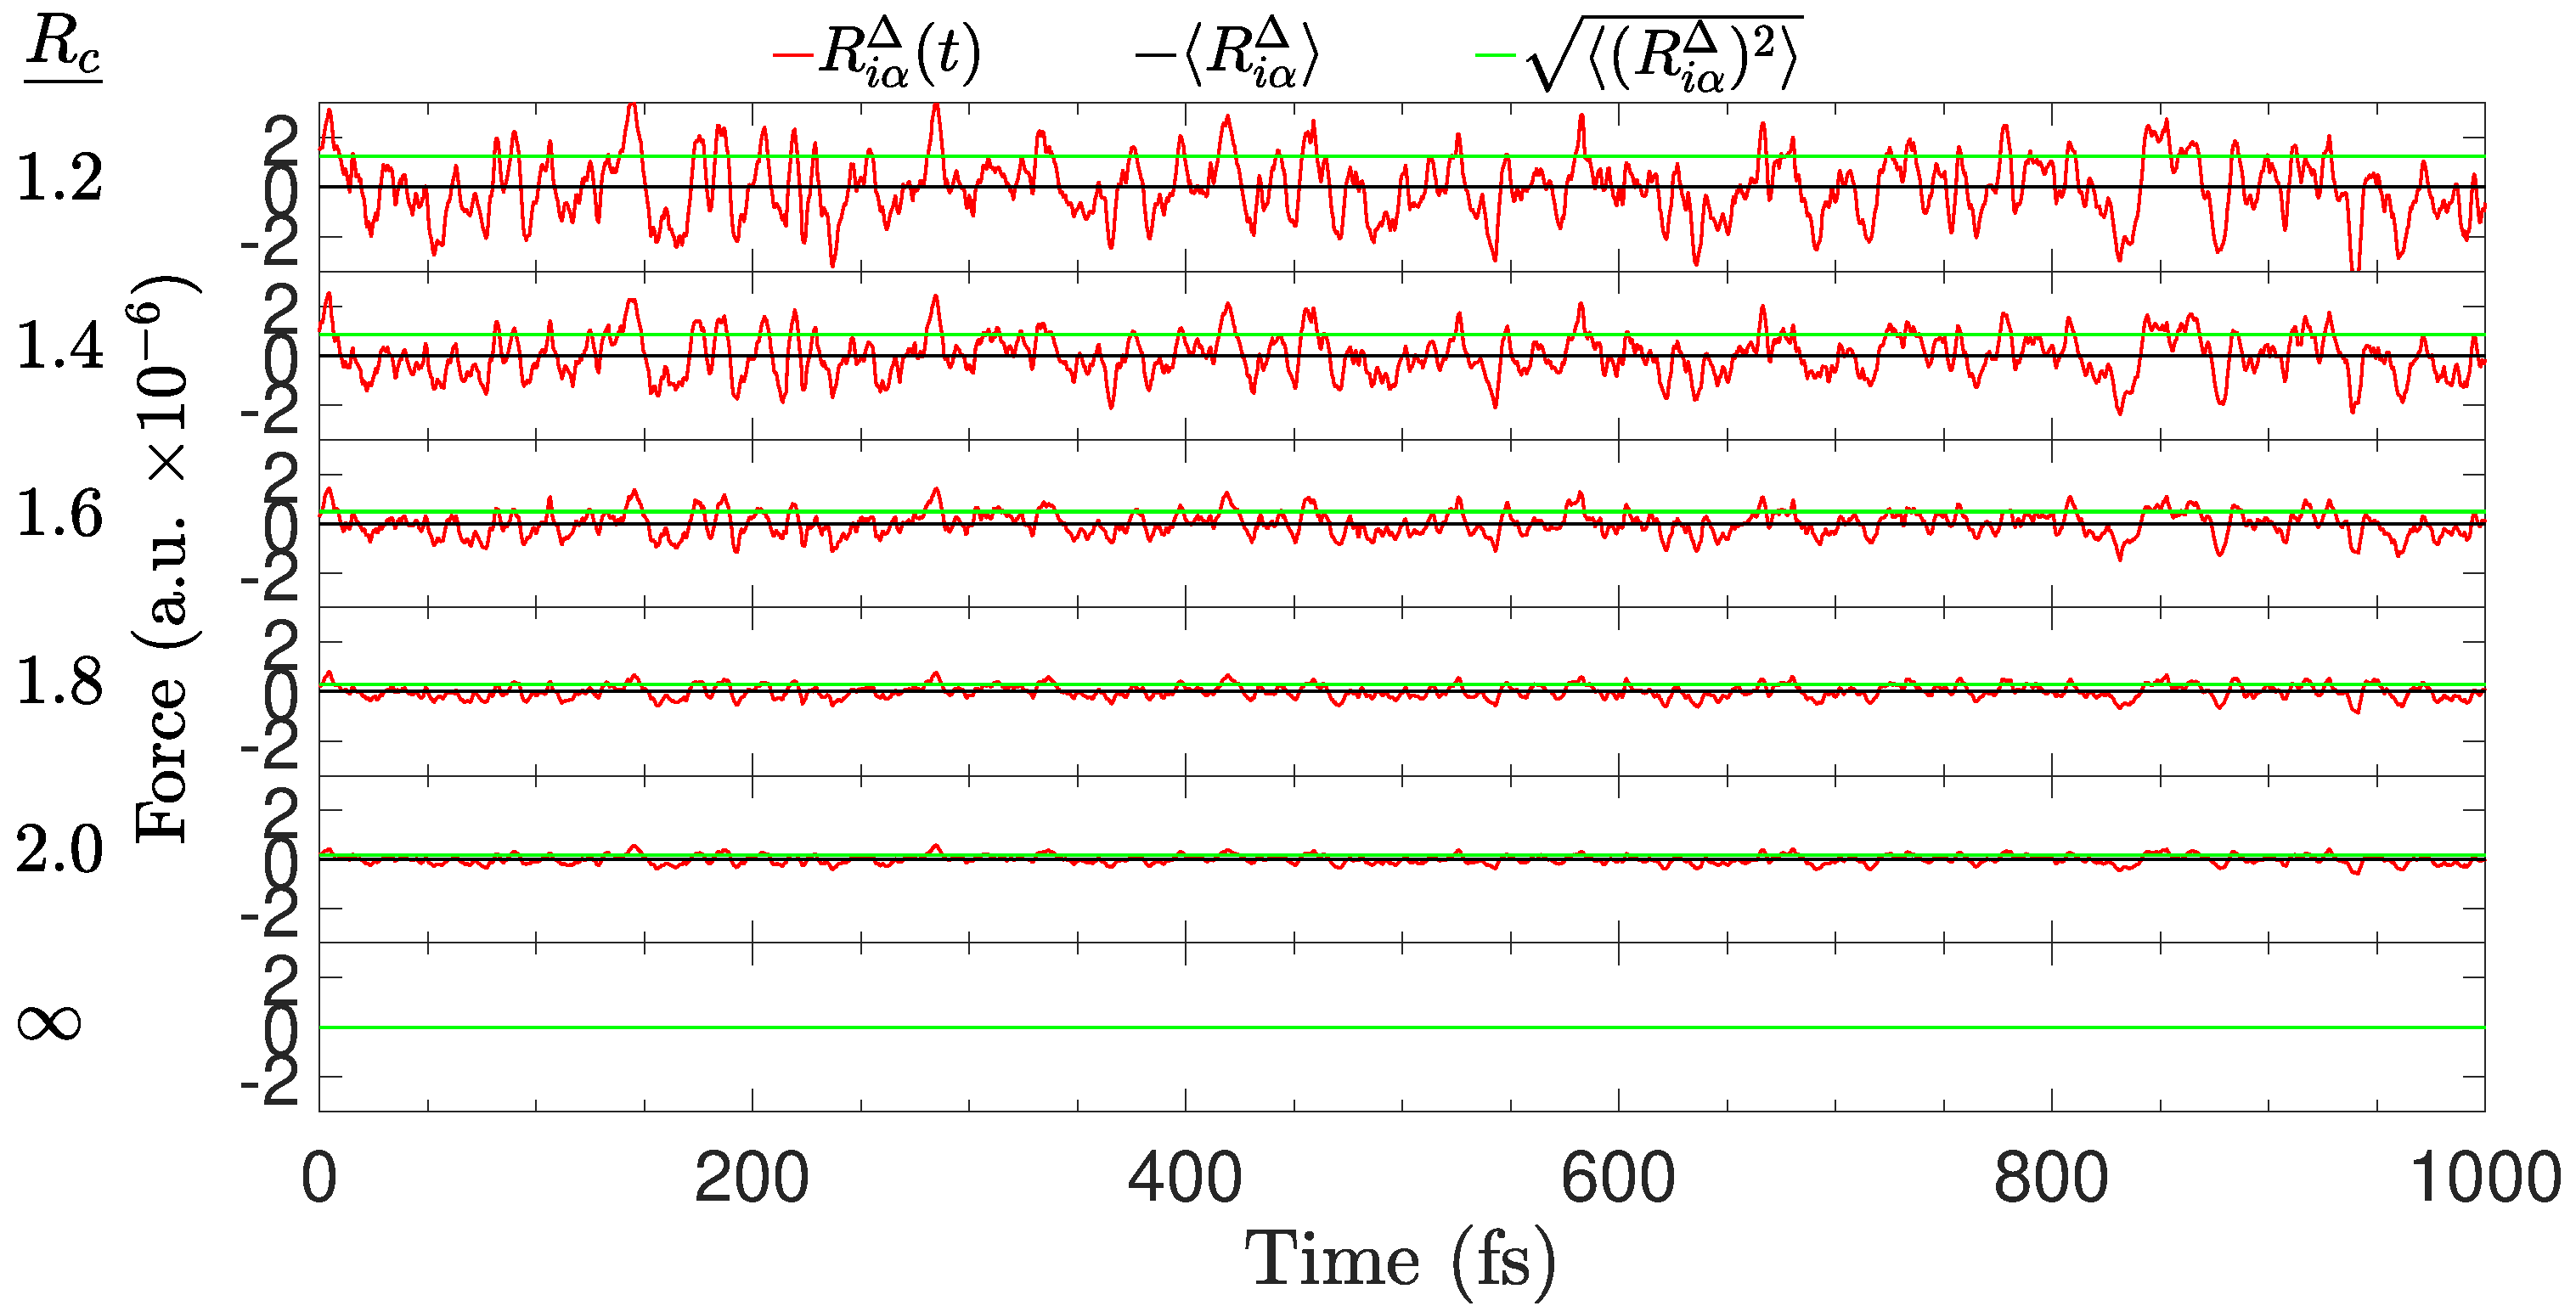
\includegraphics[trim={0.1cm 0cm 0.2cm 0.1cm},clip,width=8.6cm]{DeltaForceComparison_ALMO_SCF.eps}
\caption{\label{fig:forcecomp} {\color{red} All figures: VdWR$\rightarrow$vdWR. Hayden, your description states that you average over Cartesian components of forces. Unfortunately, averaging over components will give zero for any isotropic system observed for a sufficiently long time (i.e. for every component there will be equal but opposite component). What we would like to plot is the instantaneous magnitude of the vector force on atom/molecule, $\vert \delta \vec{f}_i(t) \vert$, averaged over all atoms/molecules.} Dependence of the instantaneous magnitude of $\vert \delta \vec{f}_i(t) \vert$ on the ALMO localization radius $R_c$. Forces are averaged over all atoms/molecules, $R_c$ is given in units of atomic van der Waals radii. %calculated as the average difference between fully converged Born-Oppenheimer forces and fully converged ALMO DFT forces, averaged over all dimensions and all molecules for each time step. Plotted are the random forces with varying localization radius $R_{c}$, .
%Here it is clear that ALMO DFT forces converge to Born-Oppenheimer forces in the limit of $R_{c} \rightarrow \infty$.
Forces are computed with the PBE XC functional, TZV2P basis set, and $\epsilon_{SCF} =ZZZ$ for configurations from a 10-ps trajectory generated with KS DFT at T=298~K.}
\end{figure}


In the present article, we propose a new approach which allows for relaxation of the constraint on $R_{c}$ by introducing related damping and stochastic terms to the force calculation by utilizing the Langevin equation of motion.~\cite{a:Kubo-1986}

\begin{align}
\label{eq:langevin}
m_i \ddot{r}_{i\alpha} = f^{\text{KS}}_{i\alpha} - \gamma m_i \dot{r}_{i\alpha} + R^{\gamma}_{i\alpha} (t),
\end{align}

Where $m_i$ refers to the mass of the i-th particle, and $r_{i\alpha}$ its position along dimension $\alpha$. 
$f^{\text{KS}}_{i\alpha}$ is the force calculated using the ALMO SCF method described above for the i-th particle along dimension $\alpha$, $\gamma$ is the Langevin scaling factor which sets the strength of both the damping term  $\gamma m_i \dot{r}_{i\alpha}$ and the stochastic Gaussian ``white noise'' term $R^{\gamma}_{i\alpha} (t)$. 
In order to correctly sample the canonical distribution, the random force must be zero mean. 
As well, the damping and white noise terms must be related by the second fluctuation dissipation theorem.~\cite{a:Kubo-1986,a:langevin-why,b:tuckerman-stat}
%
\begin{align}
\label{eq:stochastic}
\langle R^{\gamma}_{i\alpha} (t) \rangle &= 0, \\
\langle R^{\gamma}_{i\alpha} (t)  R^{\gamma}_{j\beta} (t') \rangle &= 2 k_B T \gamma m_i \delta_{ij} \delta_{\alpha\beta} \delta(t-t')
\end{align}
%
This means the damping and white noise terms will work to maintain a constant temperature while also generating the correct Maxwell-Boltzmann distribution of velocities. 

It has previously been shown that Langevin dynamics can be utilized to correct inaccurate force calculations to maintain correct dynamical properties.~\cite{a:langevin-why,a:2ndcpmd,b:tuckerman-stat,a:ceriotti} 
By utilizing Eq.\ (\ref{eq:langevin}) in conjunction with the ALMO SCF method of force calculation, we will show that discontinuity in the PES can be ignored for sufficiently large $\gamma$. 
Note that increasing $\gamma$ increases the sample size required to generate accurate dynamical properties, as more random Gaussian noise is introduced.

The concept of balancing errors in force calculation with the Langevin equation can be taken even further, thereby reducing computational overhead even more. 
During the second step of the ALMO SCF method described above, a self-consistent variational approach is taken to converge the non-orthogonal MOs. 
Generally, this step utilizes a iterative search function in order to reduce the absolute norm of the energy gradient to some target value $\epsilon_{SCF}$. 
Previously, $\epsilon_{SCF}$ had to be set very small to ensure sufficient convergence of the electron structure calculations. 
By increasing the allowable $\epsilon_{SCF}$, a great reduction in computational cost can be achieved. 
Obviously, this introduces a significant error into the calculation of forces during each time step. 
We assume that this error has the form:
%
\begin{align}
\label{eq:assumption}
f^{\text{KS}}_{i\alpha} = f^{\text{ALMO}}_{i\alpha} + R^{\Delta}_{i\alpha} (t)
\end{align}
%
where $f^{\text{KS}}_{i\alpha}$ is the force calculated from an accurate and fully converged SCF method, $f^{\text{ALMO}}_{i\alpha}$ is the approximate force calculated by allowing a large $\epsilon_{SCF}$, and $R^{\Delta}_{i\alpha} (t)$ is a stochastic ``white noise'' term that obeys
%
\begin{align}
\label{eq:stochastic2}
\langle R^{\Delta}_{i\alpha} (t) \rangle &= 0, \\
\label{eq:stochastic3}
\langle R^{\Delta}_{i\alpha} (t)  R^{\Delta}_{j\beta} (t') \rangle &= 2 k_B T \Delta m_i \delta_{ij} \delta_{\alpha\beta} \delta(t-t')
\end{align}
%
It's clear from figure \ref{fig:randomforce} that this assumption is sufficiently justified. 
Hence, the Langevin equation of motion (\ref{eq:langevin}) can be re-written with the two stochastic terms combined into one:
%
\begin{align}
\label{eq:langevin2}
m_i \ddot{r}_{i\alpha} = f^{\text{ALMO}}_{i\alpha} - \gamma m_i \dot{r}_{i\alpha} + R^{\gamma + \Delta}_{i\alpha} (t)
\end{align}
%
where $R^{\gamma + \Delta}_{i\alpha} = R^{\gamma}_{i\alpha} + R^{\Delta}_{i\alpha}$. 
Note that $\Delta$ can be either positive or negative depending on the way errors are introduced in the system of interest. 
$\Delta$ was found to be positive for all systems considered here, increasing the amplitude of the effective random force on the system.

%\section{Optimizing the values of $\gamma$ and $\Delta$}

In theory, both $\gamma$ and $\Delta$ should be system-size independent, but in practice only $\gamma$ is.
We found that $\Delta$ is dependent on system size due to finite size effects, which decay for increasing system size.
Fortunately, $\gamma$ and $\Delta$ can be separately optimized for a given system of interest, assuming a method of accurate force calculation can be applied to the system for a short trajectory. 

An optimized $\gamma$ is one that is: large enough to adequately absorb force discontinuities; large enough to correctly thermostat the system of interest on a reasonable time scale; and small enough not to significantly affect dynamical properties on the time scale of interest. 
The relative weight of the three is determined by the specifics of the system and what is most important to the researcher. 
To optimize $\gamma$ given the relative importance of the above properties, we suggest running several short trajectories on the system of interest (or a scaled-down version of it) using a tightly converged PES calculation and varying the value of $\gamma$. 
We found that a value of $\gamma$ between $10^{-5}$ and $10^{-3}\ \mathrm{fs^{-1}}$ was optimal for the purposes of the research presented here.

To correctly thermostat the system of interest, $\Delta$ needs to be reduced to zero.
This is done by finding the value of $\Delta$ and adding a third random force term $R^{-\Delta}_{i\alpha}$ to equation \ref{eq:langevin2} which cancels out the energy introduced to the system by $R^{\Delta}_{i\alpha}$.
This means that a trajectory with inaccurate forces and optimized $R^{-\Delta}_{i\alpha}$ should have no long term drift in the total energy of the system. 
Short term energy fluctuations should be expected, and can later be ``smoothed out'' by setting finite $\gamma$.

$R^{-\Delta}_{i\alpha}$ can therefore be optimized simply by trying various values of $\Delta$ (with \mbox{$\gamma = 0$}) until the simulation has long-term stable total energy and satisfies the equipartition theorem. 
%
\begin{align}
\label{eq:eqipartition}
\langle \dfrac{1}{2} m_i \dot{\bm{r}}^{2}_{i} \rangle &= \dfrac{3}{2} k_{B} T
\end{align}
%

Another approach based on Eq. (\ref{eq:assumption}) can be used to find $\Delta$ within an order of magnitude if one can afford computing tightly converged SCF forces for a short MD trajectory. 
First, run the simulation with $\Delta = 0$ and converged SCF forces. 
Second, compute approximate forces for snapshots along the trajectory and calculate the random term $R^{\Delta}_{i\alpha} (t)$ using Eq.\ \ref{eq:assumption}. 
Third, calculate the autocovariance function (ACF) of the noise $\text{ACF}(t) = \langle R^{\Delta}_{i\alpha} (0)  R^{\Delta}_{i\alpha} (t) \rangle$, which should be sharply peaked around zero lag time if our assumption is correct. 
Finally, integrate Eq.(\ref{eq:stochastic3}) to obtain the following expression for $\Delta$.
%
\begin{align}
\label{eq:delta}
\Delta &= (2 k_B T m_i )^{-1} \int_{-\infty}^{\infty}\langle R^{\Delta}_{i\alpha} (0)  R^{\Delta}_{i\alpha} (t) \rangle dt
\end{align}
%
In other words, we use the integral of the ACF to estimate the strength of the random force. 
In practice, we found this method for estimating $\Delta$ was not particularly accurate due to rapidly oscillating correlations between sequential values of $R^{\Delta}_{i\alpha} (t)$. 
The ACF was not possible to accurately integrate without running a reference trajectory with extremely short time-steps (see figure~\ref{fig:randomforce}).
For example, using Eq.\ \ref{eq:delta} we calculated $\Delta \approx \SI{2e-5}{\per\fs}$, but value was optimized heuristically to $\SI{6e-5}{\per\fs}$.
Still, this method provided a decent order of magnitude starting point for further investigation.
Note that for our system, the ACF decays rapidly enough that the forces can be considered random and uncorrelated to a good approximation for sufficiently long time scales ($\gg\SI{200}{\fs}$).

\begin{figure}
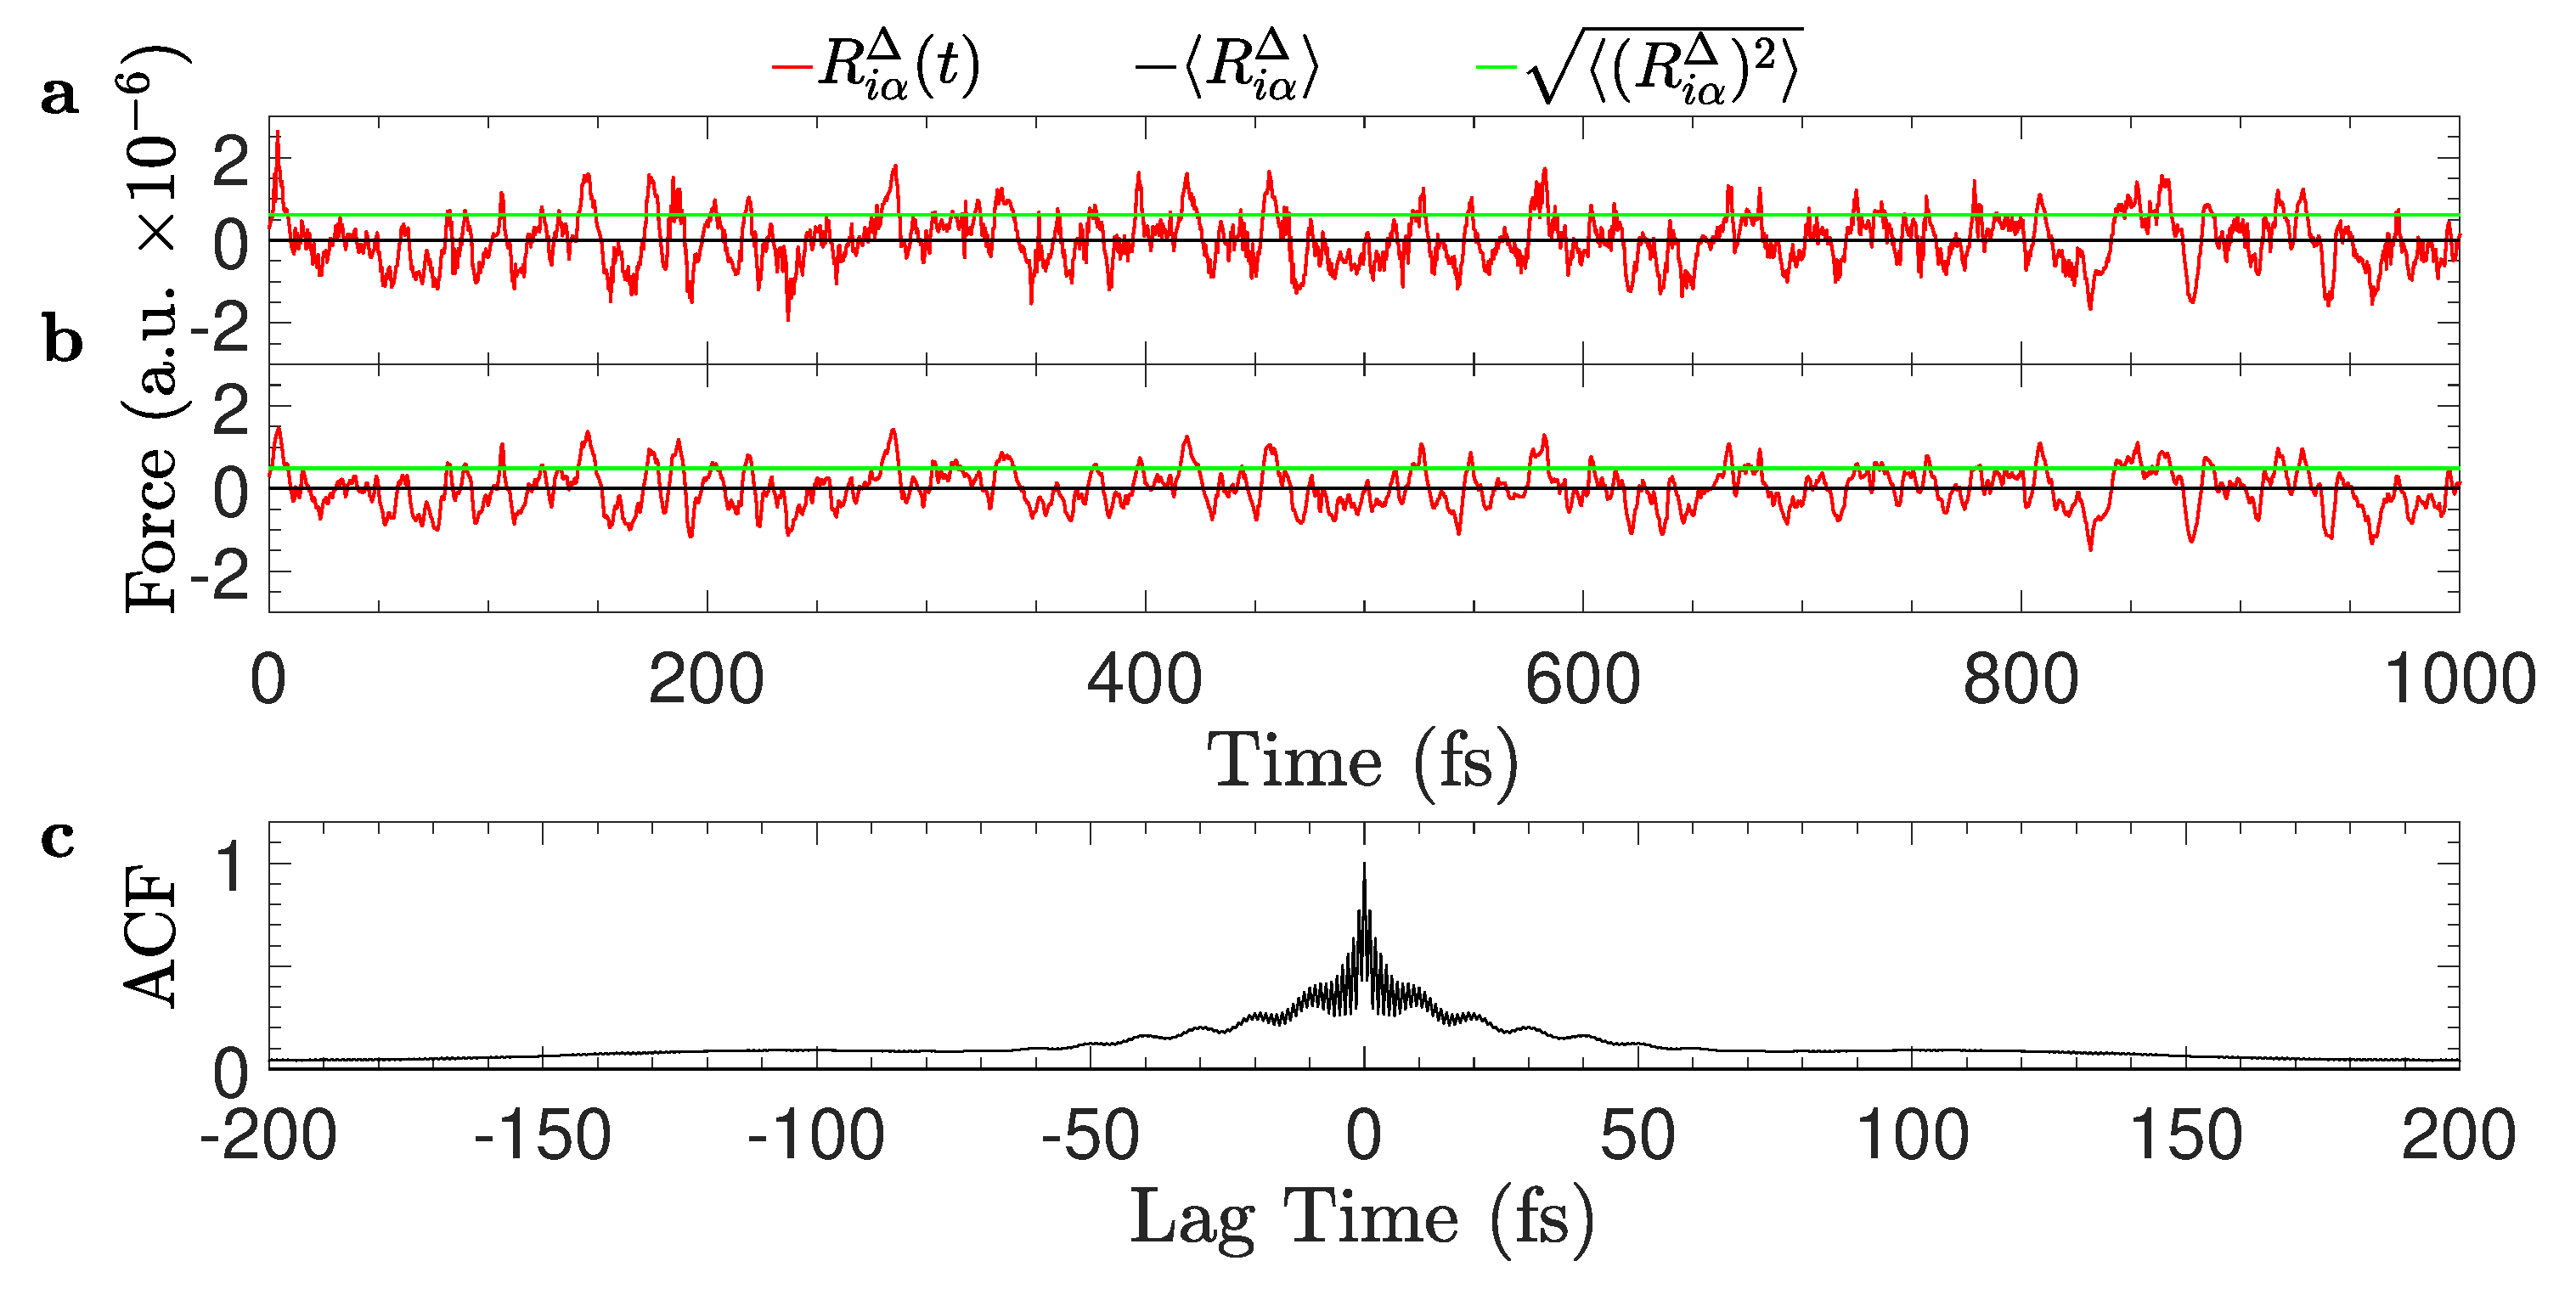
\includegraphics[trim={0.6cm 0.7cm 0.7cm 0.3cm},clip,width=8.6cm]{DeltaForceComparison_with_ACF.eps}
\caption{\label{fig:randomforce}The ``Random force'' along a water molecule dimension $\langle R^{\Delta}_{i\alpha} \rangle (t)$ calculated as the difference between the fully converged Born-Oppenheimer forces and ALMO DFT forces. Here it is clear that Eq.\ (\ref{eq:stochastic2}) is satisfied. 
(a) Plot of $\langle R^{\Delta}_{i\alpha} \rangle (t)$ as a function of time, where $R_{C} = 1.6$ VdWR and $\epsilon_{SCF} = 10^{-2}$.
(b) Plot of $\langle R^{\Delta}_{i\alpha} \rangle (t)$ as a function of time, where $R_{C} = 1.6$ VdWR and forces are fully converged.
(c) Autocorrelation function of plot a, $\langle R^{\Delta}_{i\alpha} (t) R^{\Delta}_{i\alpha} (t+\tau) \rangle $. 
Calculations were performed with the PBE $\mathrm{E_{XC}}$ functional and the TZV2P basis set on 125 water molecules for 10 ps at 298 K.}
\end{figure}

%\section{Implementation}

The methods presented here are built into CP2K, an open source MD simulation package.~\cite{www:cp2k} 
The computation scheme used is mostly identical to that described in the implementation section of ref.\ \citenum{a:almo-ls}. 
For the dynamical properties calculations using ALMO DFT methods, a periodic cell containing 125 water molecules was simulated for $\SI{10}{\ps}$ at a temperature of $\SI{293}{\K}$ and a constant density of $\SI{1.00597}{\g\per\cm^{3}}$. 
The system was thermostated using the Langevin ensemble (eq.\ \ref{eq:langevin2}) where $\gamma$ was set to $\SI{e-3}{\per\fs}$, and $\Delta$ was optimized to the order of $10^{-5}\, \mathrm{fs^{-1}}$. 
Note that for timing benchmarks, $\Delta$ was not optimized. 
This does not have a perceptible effect on calculation time.

Simulations for timing benchmarks were run for ten time steps, which is sufficient for convergence of wavefunctions from an initial guess.
The TZV2P basis set was used to represent MOs, and a cutoff of $\SI{320}{Ry}$ used to represent electron density. 
The exchange-correlation energy was approximated using the PBE functional, which expands upon the local density approximation by considering derivatives of the electron density at each point.~\cite{a:PBEfunctional} 

The reference PES was calculated using the orbital transformation (OT) method~\cite{a:ot,a:ot2} at $\SI{302}{\K}$ and the Langevin thermostat with $\gamma = \SI{e-3}{\per\fs}$. 
All other system parameters were set identical to the ALMO system.

IR spectra, radial distribution functions, diffusivity plots, and diffusion constants were calculated using the open source trajectory analyzer program TRAVIS.~\cite{a:travis-main,a:travis-ir1,a:travis-ir2}

%\section{Accuracy}

In order to confirm that ALMO DFT forces are accurate in the limit where localization radius $R_{c} \rightarrow \infty$, we computed the average difference in force between fully converged Born-Oppenheimer forces and forces calculated from ALMO DFT with varying $R_{c}$. 
Figure \ref{fig:forcecomp} shows that as $R_{c}$ is increased to infinity, forces converge toward the Born-Oppenheimer limit.

To test the accuracy of our unconverged ALMO based MD we computed the Infrared (IR) spectrum, radial distribution function (RDF), kinetic energy distribution, and mean-squared displacement (MSD) function from a 10 ps MD trajectory (see fig. \ref{fig:dynproperties} and the Supplemental Material). 
We compared the IR spectrum, RDF, and MSD function to corresponding reference functions calculated with fully converged KS DFT forces.
The kinetic energy distribution is compared with the theoretical Maxwell-Boltzmann distribution at the average temperature of the system.
From the slope of the MSD functions we also calculated diffusion constants.
Using fully converged KS DFT forces we calculated D = $\SI{5.47e-9}{\m^{2}\per\s}$, whereas with unconverged ALMO forces we calculated D = $\SI{5.55E-09}{\m^{2}\per\s}$.

Although the accuracy of calculated properties in figure \ref{fig:dynproperties} is quite good, it is clear that there are errors present.
Some of the error can be attributed to the 9 K difference in the thermodynamic temperature between the reference system and our system of interest.
Other sources of error are: small temporal sample size given our choice of $\gamma$; random error due to finite localization radius $R_{c}$, and random error due to high $\epsilon_{SCF}$.
From figure \ref{fig:randomforce}, it's apparent that high values of $R_{c}$ introduce more random error than high values of $\epsilon_{SCF}$.
However, raising both $R_{c}$ and $\gamma$ decreases computation time significantly, and it is ultimately up to the user to determine their maximum tolerance of force inaccuracy when using ALMO DFT methods.

\begin{figure}
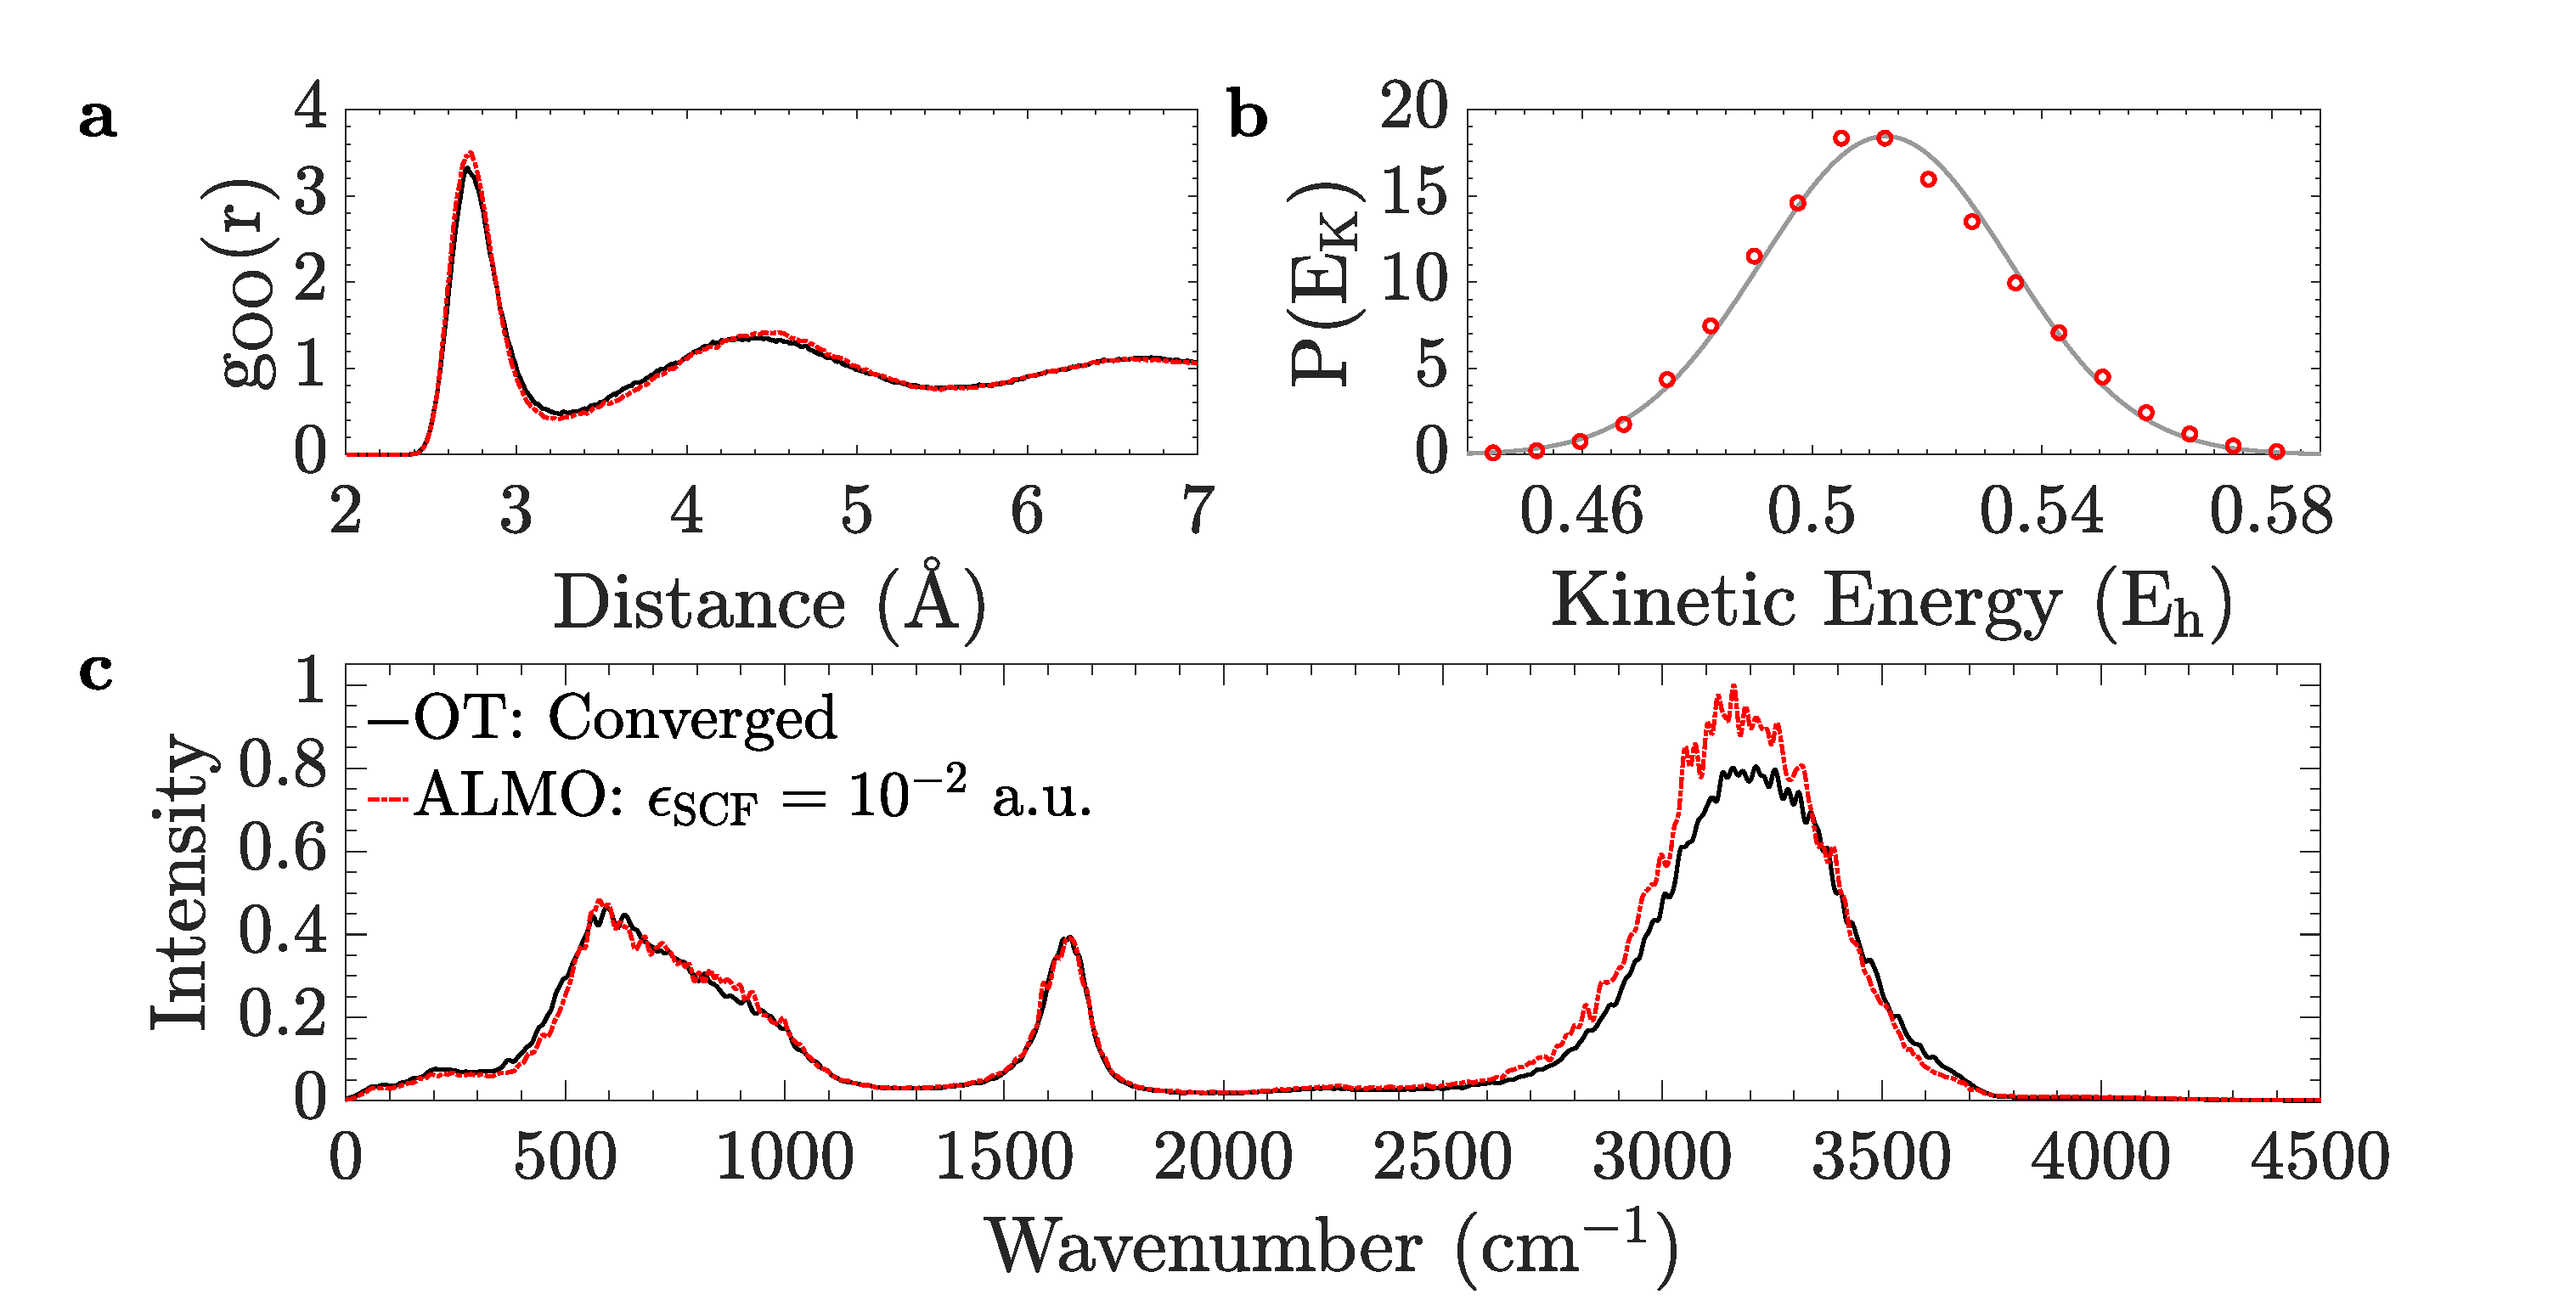
\includegraphics[trim={1.3cm 0.1cm 3.3cm 1.3cm},clip,width=8.6cm]{Dynamical_Data_Tiled.eps}
\caption{\label{fig:dynproperties} Calculated dynamic and static properties of water using ALMO DFT with $\epsilon_{SCF} = 10^{-2}$ and $R_{c} = 1.6$ VdWR.
(a) Radial distribution function of an ALMO simulation compared to OT SCF with a fully converged PES. 
(b) Kinetic energy distribution of an ALMO simulation compared to the theoretical Maxwell-Boltzmann kinetic energy distribution.
(c) Calculated Infrared spectrum of an ALMO simulation compared to OT SCF with a fully converged PES.
Calculations were performed with the PBE $\mathrm{E_{XC}}$ functional and TZV2P basis set, using 125 water molecules for 10 ps.}
\end{figure}

%\section{Speed}

To show the computational efficiency gained by using unconverged ALMO DFT forces, we compare the average wall-time per MD step over 10 time steps for various values of $\epsilon_{SCF}$ in figure \ref{fig:strongscaling_log}.
For these simulations, we chose to set the localization radius $R_{c} = 1.6$ Van der Waal Radii (VdWR), as was done for calculation of dynamical properties.
We also show timing of the fully converged OT SCF method, as well as the recently developed ``second generation Car-Parinello'' MD method, which improves upon the OT computational cost prefactor.~\cite{a:2ndcpmd}
ALMO methods show clear asymptotic LS behavior for all values of $\epsilon_{SCF}$ tested.
OT SCF scales approximately cubically, as expected.
Our findings show that the fastest ALMO DFT method presented here runs faster than second-generation Car-Parinello using OT DFT for water simulations larger than 256 molecules.

\begin{figure}
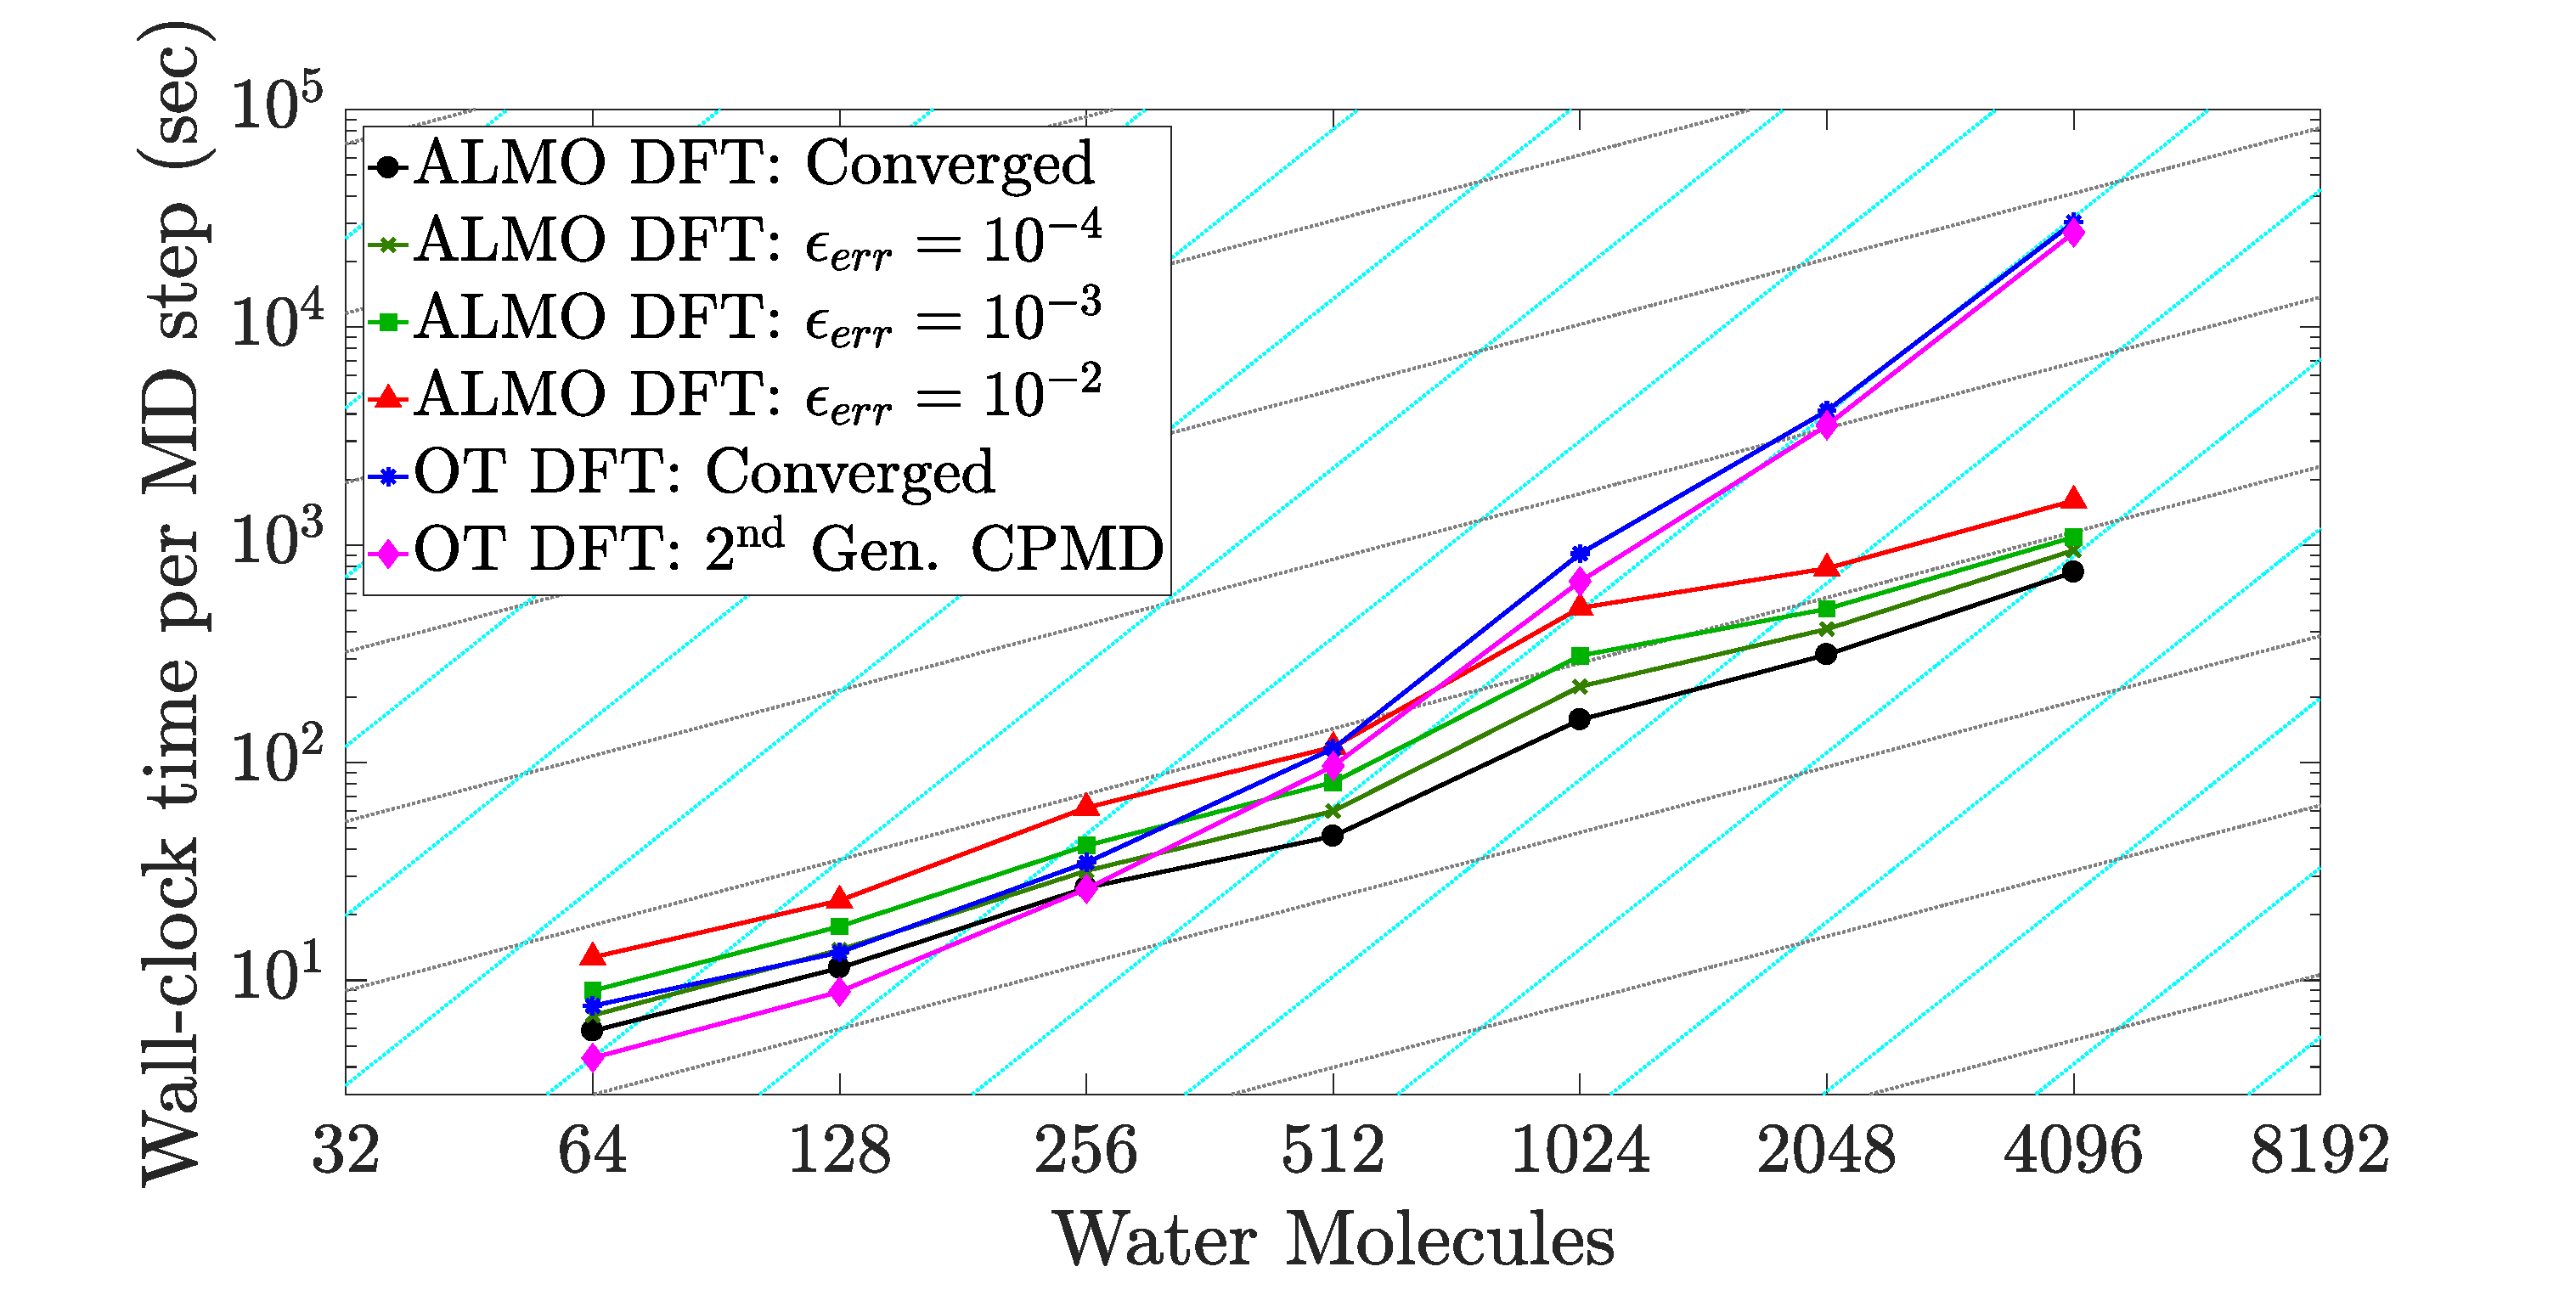
\includegraphics[trim={2.5cm 0.5cm 3.4cm 0.1cm},clip,width=8.6cm]{strongscaling_log.eps}
\caption{\label{fig:strongscaling_log} Logscale plots which show the asymptotic LS behaviour of ALMO methods for liquid water at 298 K.
Compared with the orbital transformation using fully converged SCF and second generation Car-Parinello force calculation methods.~\cite{a:ot,a:ot2,a:2ndcpmd}
Cyan lines represent perfect cubic scaling, whereas gray lines represent perfect linear scaling. 
Calculations were performed with the PBE $\mathrm{E_{XC}}$ functional and TZV2P basis set on 256 cores, averaged over 10 MD steps. 
The localization radius was set to $R_{c} = 1.6$ VdWR.}
\end{figure}

Figure \ref{fig:weakscaling} shows that ALMO MD code is well optimized for parallelization, and that computational cost grows linearly under a wide range of available computing power. 
In fact, we were able to successfully simulate systems as large as 32768 water molecules within 25 minutes of wall-clock time using 4096 cores.

%\begin{figure}
%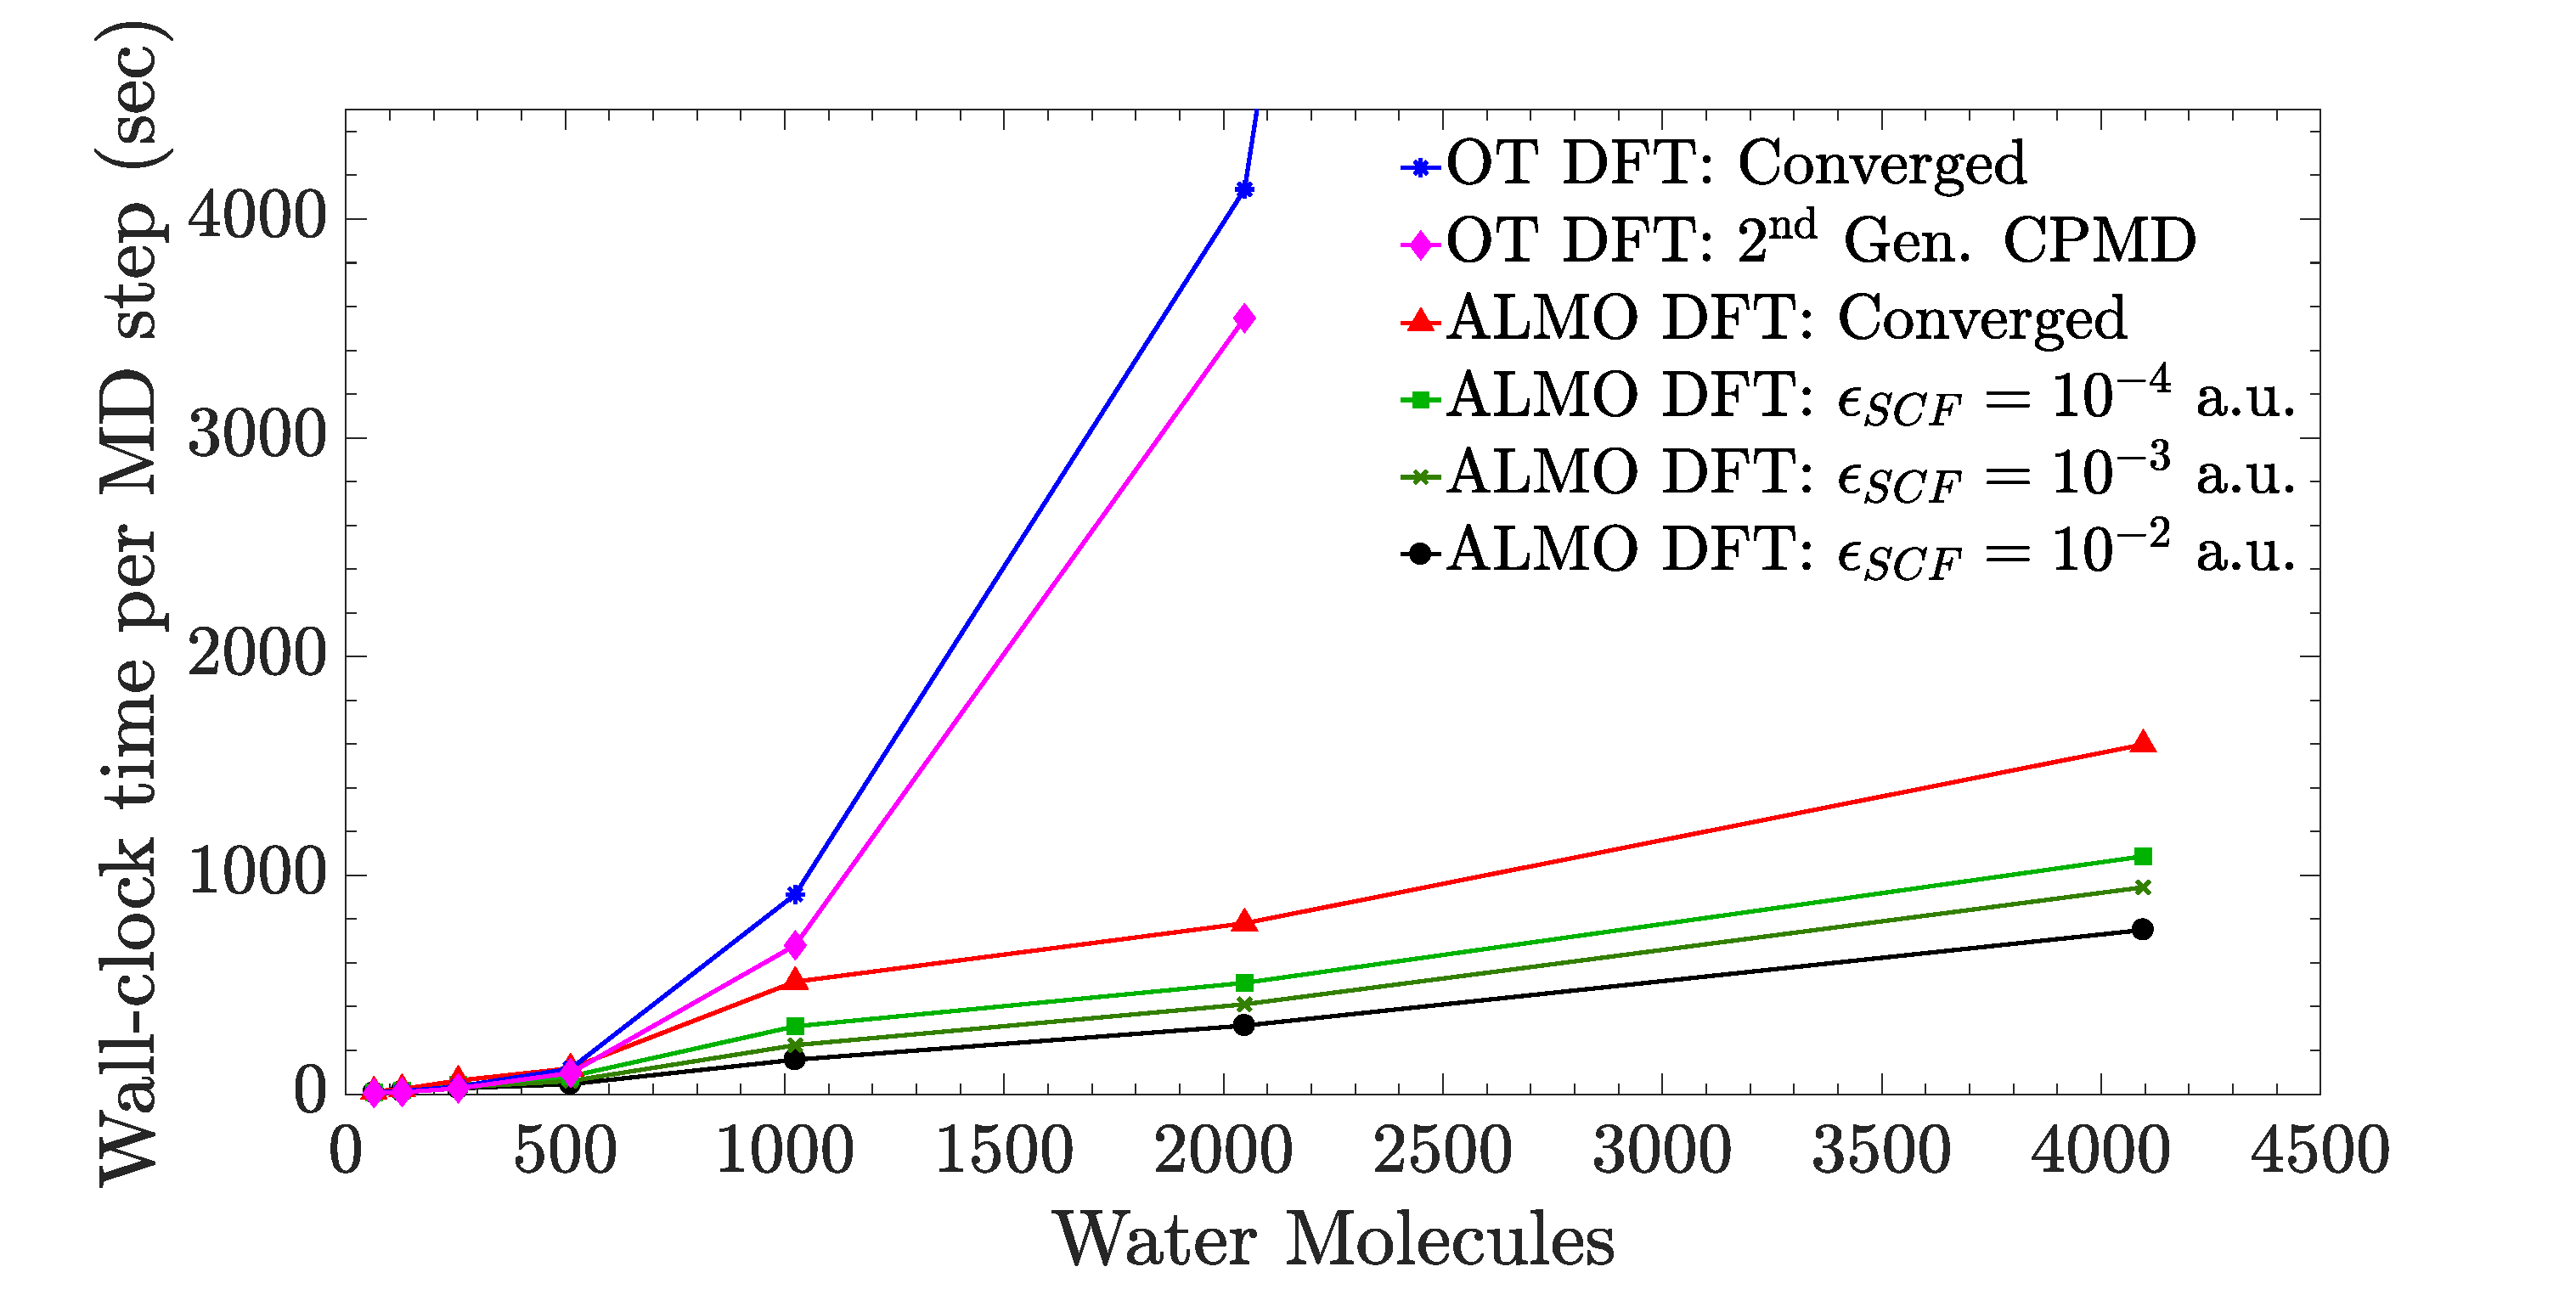
\includegraphics[trim={1.7cm 0.5cm 3.3cm 0.1cm},clip,width=8.6cm]{strongscaling_linear.eps}
%\caption{\label{fig:strongscaling_linear} Linear plots showing LS behaviour of all ALMO methods for liquid water at 298 K. 
%Calculations were performed with the PBE $\mathrm{E_{XC}}$ functional and TZV2P basis set on 256 cores. 
%The localization radius was set to $R_{c} = 1.6$ VdWR.}
%\end{figure}

\begin{figure}
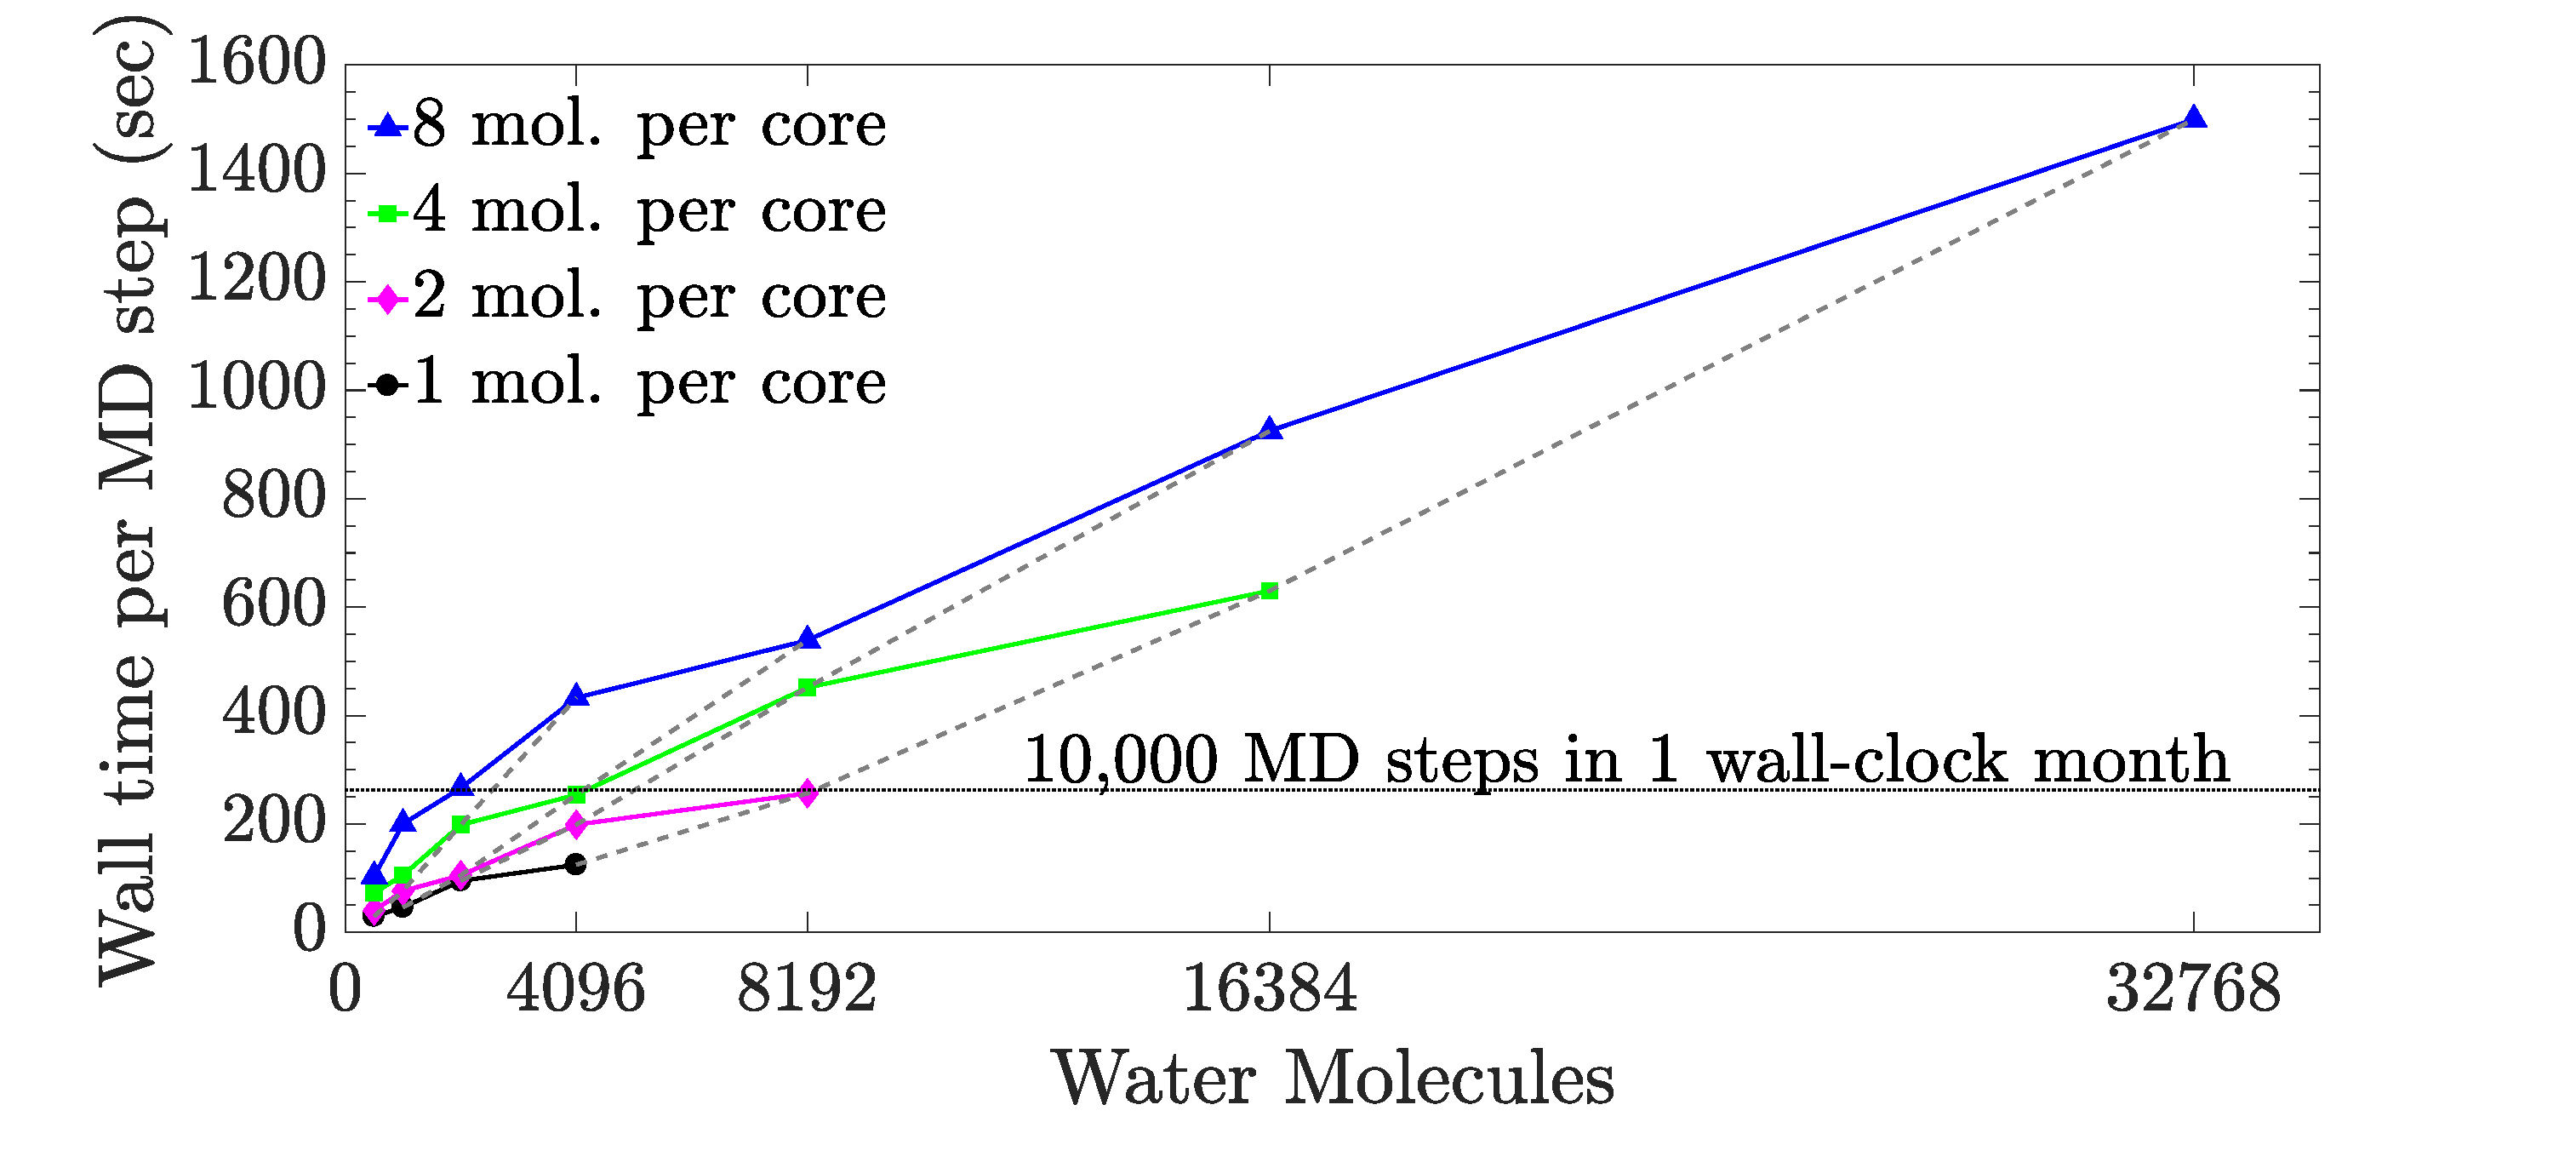
\includegraphics[trim={1.6cm 0cm 4.7cm 0cm},clip,width=8.6cm]{weakscaling.eps}
\caption{\label{fig:weakscaling} Weak scalability benchmarks showing optimization of code for parallel computing.
Dashed gray lines connect systems simulated using the same number of cores, verifying LS behaviour over a range of configurations.
Of note is the 32768 molecule system successfully simulated using 4096 cores at around 25 minutes per MD step.
We also show that systems as large as 8192 molecules can be simulated for 10,000 MD steps in under a month using this method.
Calculations were performed with the PBE $\mathrm{E_{XC}}$ functional and TZV2P basis set, averaged over 10 MD steps. 
The localization radius was set to $R_{c} = 1.6$ VdWR and $\epsilon_{SCF} = 10^{-2}$.}
\end{figure}

%\section{Conclusions} 

In this article we have clearly demonstrated the utility of ALMO DFT methods, especially when combined with the Langevin Equation of motion.
ALMO DFT methods are a powerful class of AIMD electronic structure determination techniques capable of efficiently calculating forces for weakly coupled molecular systems.
It's clear that forces calculated by ALMO DFT can be tuned as accurately as required by the user, up to the Born-Oppenheimer limit.
Indeed, the ALMO DFT technique highlighted in this article has been shown to be capable of producing potential energy surfaces extremely efficiently for medium to large systems with only a minimal drop in the accuracy of calculated bulk system properties.
We have also shown that due to its linear scaling nature, the ALMO DFT technique can be pushed to simulate enormous chemical systems accurately in remarkably short calculation times.

To summarize, a low-cost linear-scaling AIMD method for weakly-interacting molecular systems was developed by utilizing compact molecular orbitals strictly localized within predefined radii. High efficiency of the method is achieved without sacrificing its accuracy with a combination of two techniques: (1) on-the-fly construction of accurate localized orbitals without lengthy self-consistent optimization and (2) a modified Langevin equation that is fine-tuned to retain stable dynamics even with imperfect forces. A remarkable feature of the implemented method is that it remains efficient for challenging condensed phase systems, even with diffuse atom-centered basis sets. Using liquid water as an example, it is demonstrated that the new AIMD method enables simulations of molecular systems on previously inaccessible time and length scales. 

Generalization of the method to more challenging systems of strongly interacting atoms (e.g. covalent crystals) will also be discussed.

%Such simulations are important for Use if empirical force fields or QM/MM are not applicable:
%Chemical reactions that happen throughout your system, not in a localized spatial region (e.g. proton transfer in water)
%Unusual thermodynamic states for which simple analytical potential become inaccurate (e.g. high pressure states, interfaces, heterojunctions)
%Electron density is an important observable (e.g. X-ray scattering) or information of the electronic wavefunctions is crucial.


\textbf{Acknowledgments.} The research was funded by the Natural Sciences and Engineering Research Council of Canada through the Discovery Grant. The authors are grateful to Compute Canada and McGill HPC Centre for computer time.

%\textbf{Supplemental Material}

%ZZZ outline procedure to compute forces using the DM obtained from ALMOs.
% ZZZ figure to show 

\bibliography{almo-langevin}

\end{document}
